% Grand Rosetta Table - Auto-generated
\begin{table}[htbp]
\centering
\caption{Complete classification of Rosetta Stone PCF families. All families share $a_n = (k_0 + 2m\sigma)n - 2n^2$, $b_n = \varepsilon + 3n$. The telescoping condition $\alpha - \beta \in \mathbb{Z}$ causes all transcendental factors to cancel.}
\label{tab:rosetta}
\begin{tabular}{cccccccll}
\toprule
Fam & Label & $\alpha$ & $\beta$ & $\alpha{-}\beta$ & $V(0)$ & Ratio & Closed Form & Type \\
\midrule
1 & $T^{(m+1)}$ & $3/2$ & $1/2$ & $1$ & $3$ & $\frac{m+3/2}{m+1/2}$ & $2m + 3$ & Telescoping \\
2 & $T^{(m)}$ & $1/2$ & $-1/2$ & $1$ & $1$ & $\frac{m+1/2}{m-1/2}$ & $2m + 1$ & Telescoping \\
3 & $S^{(m+1)}$ & $1$ & $1/2$ & $1/2$ & $\frac{4}{\pi}$ & $\frac{m+1}{m+1/2}$ & $S^{(m+1)}$ & $S$-shift ($\mathbb{Z}$) \\
4 & $S^{(m+3/2)}$ & $3/2$ & $1$ & $1/2$ & $\frac{3}{2}$ & $\frac{m+3/2}{m+1}$ & $S^{(m+3/2)}$ & $S$-shift ($\mathbb{Z}$) \\
\midrule
\multicolumn{9}{p{0.92\linewidth}}{\textbf{Experiment log (2026-04-09):} Fractional $\beta$ sweep over reduced $p/q$ with $1 \le q \le 12$, $|\beta| \le 3$, and $\gcd(p,q)=1$ (266 cases). Best cubic candidates reached $81.1{+}$ stable digits, but no PSLQ relation was found in the rational, $\Gamma(1/3)$, or $\Gamma(2/3)$ sectors; the $\Gamma(1/4)$ and $\Gamma(3/4)$ sectors remain under-resolved.} \\
\bottomrule
\end{tabular}
\end{table}

% ── Phase Diagram: Dichotomy Principle ────────────────────────────────────
% Requires: \usepackage{tikz} and \usepackage{pgfplots} in preamble
\begin{figure}[htbp]
\centering
\begin{tikzpicture}[
    >=latex,
    every node/.style={font=\small},
    rational/.style={line width=2pt, blue!70!black},
    transcendental/.style={line width=1.4pt, dashed, red!70!black},
    fampoint/.style={circle, inner sep=2.2pt, fill},
    famlabel/.style={font=\footnotesize\bfseries, anchor=south west, inner sep=2pt},
]

% ── Coordinate scaling ──
\def\xscale{3.2}   % horizontal stretch
\def\yscale{2.6}   % vertical stretch

% ── Background shading for zones ──
% Integer-gap band (rational)
\fill[blue!6] (-0.4*\xscale, 0.75*\yscale) rectangle (2.6*\xscale, 1.25*\yscale);
\fill[blue!6] (-0.4*\xscale, 1.75*\yscale) rectangle (2.6*\xscale, 2.25*\yscale);
% Half-integer-gap band (transcendental)
\fill[red!6]  (-0.4*\xscale, 0.25*\yscale) rectangle (2.6*\xscale, 0.75*\yscale);
\fill[red!6]  (-0.4*\xscale, 1.25*\yscale) rectangle (2.6*\xscale, 1.75*\yscale);

% ── Axes ──
\draw[->] (-0.5*\xscale, 0) -- (2.8*\xscale, 0)
    node[right, font=\normalsize] {Parameter~$(m)$};
\draw[->] (-0.4*\xscale, -0.15*\yscale) -- (-0.4*\xscale, 2.4*\yscale)
    node[above, font=\normalsize] {Gap~$(\alpha - \beta)$};

% ── Y-axis tick labels ──
\foreach \y/\lab in {0/$0$, 0.5/$\tfrac{1}{2}$, 1/$1$, 1.5/$\tfrac{3}{2}$, 2/$2$} {
    \draw (-0.4*\xscale - 3pt, \y*\yscale) -- (-0.4*\xscale + 3pt, \y*\yscale);
    \node[left, font=\small] at (-0.4*\xscale - 4pt, \y*\yscale) {\lab};
}

% ── X-axis tick labels ──
\foreach \x in {0, 1, 2} {
    \draw (\x*\xscale, -3pt) -- (\x*\xscale, 3pt);
    \node[below, font=\small] at (\x*\xscale, -5pt) {$\x$};
}

% ── Horizontal zone lines ──
% Rational (integer gap) — solid thick
\draw[rational] (-0.3*\xscale, 1*\yscale) -- (2.5*\xscale, 1*\yscale);
\draw[rational] (-0.3*\xscale, 2*\yscale) -- (2.5*\xscale, 2*\yscale);
\node[blue!70!black, font=\footnotesize, anchor=west]
    at (2.55*\xscale, 1*\yscale) {Rational ($T$-type)};
\node[blue!70!black, font=\footnotesize, anchor=west]
    at (2.55*\xscale, 2*\yscale) {Rational ($T$-type)};

% Transcendental (half-integer gap) — dashed
\draw[transcendental] (-0.3*\xscale, 0.5*\yscale) -- (2.5*\xscale, 0.5*\yscale);
\draw[transcendental] (-0.3*\xscale, 1.5*\yscale) -- (2.5*\xscale, 1.5*\yscale);
\node[red!70!black, font=\footnotesize, anchor=west]
    at (2.55*\xscale, 0.5*\yscale) {Transcendental ($S$-type)};
\node[red!70!black, font=\footnotesize, anchor=west]
    at (2.55*\xscale, 1.5*\yscale) {Transcendental ($S$-type)};

% ── Family discovery points ──
% Family 2: T^(m), alpha=1/2, beta=-1/2, gap=1  — plotted at user-specified (0, 1/2)
% Family 1: T^(m+1), alpha=3/2, beta=1/2, gap=1 — plotted at user-specified (0, 3/2)
% Family 3: S^(m+1), alpha=1, beta=1/2, gap=1/2 — plotted at user-specified (1/2, 1)
% Family 4: S^(m+3/2), alpha=3/2, beta=1, gap=1/2 — plotted at user-specified (3/2, 3/2)

% --- Data-faithful alternative (α−β on Y): ---
% Family 2 — T^(m): gap = 1
\node[fampoint, blue!70!black] (F2) at (0*\xscale, 1*\yscale) {};
\node[famlabel, blue!70!black, anchor=north east]
    at ([xshift=-2pt, yshift=-1pt] F2) {Fam\,2: $T^{(m)}$};

% Family 1 — T^(m+1): gap = 1
\node[fampoint, blue!70!black] (F1) at (0.35*\xscale, 1*\yscale) {};
\node[famlabel, blue!70!black, anchor=south west]
    at ([xshift=2pt, yshift=1pt] F1) {Fam\,1: $T^{(m+1)}$};

% Family 3 — S^(m+1): gap = 1/2
\node[fampoint, red!70!black] (F3) at (1*\xscale, 0.5*\yscale) {};
\node[famlabel, red!70!black, anchor=south west]
    at ([xshift=2pt, yshift=1pt] F3) {Fam\,3: $S^{(m+1)}$};

% Family 4 — S^(m+3/2): gap = 1/2
\node[fampoint, red!70!black] (F4) at (1.5*\xscale, 0.5*\yscale) {};
\node[famlabel, red!70!black, anchor=north west]
    at ([xshift=2pt, yshift=-1pt] F4) {Fam\,4: $S^{(m+\frac{3}{2})}$};

% ── Dashed zero line ──
\draw[gray!40, thin] (-0.3*\xscale, 0) -- (2.5*\xscale, 0);

% ── Annotation: dichotomy rule ──
\node[draw, rounded corners=3pt, fill=white, inner sep=5pt,
      font=\footnotesize, text width=5.8cm, align=center]
    at (1*\xscale, -0.65*\yscale)
    {$\alpha - \beta \in \mathbb{Z}$~\raisebox{0.5pt}{\tikz\draw[blue!70!black,line width=1.5pt](0,0)--(0.5,0);}~\,Rational
     \quad\textbar\quad
     $\alpha - \beta \in \mathbb{Z}{+}\tfrac{1}{2}$~\raisebox{0.5pt}{\tikz\draw[red!70!black,dashed,line width=1.2pt](0,0)--(0.5,0);}~\,Transcendental};

\end{tikzpicture}
\caption{The structure of PCF convergence types.
Rational solutions coalesce on integer gaps
($\alpha - \beta \in \mathbb{Z}$, solid blue),
while transcendental values emerge at half-integer shifts
($\alpha - \beta \in \mathbb{Z} + \tfrac{1}{2}$, dashed red),
generalised by the unique signature of the $S$-family.
Shaded bands indicate the predicted continuation of each zone
to higher gap values.}
\label{fig:dichotomy}
\end{figure}
